\section{Experiments}
%
In this section we describe the experiments carried out in order to assess 
the performance and the behavior of our extended kitchen sinks (\eks) and 
unscented kitchen sinks (\uks) methods. We first look at experiments on 
small-scale synthetic inversion problems and a binary classification task on 
the \usps dataset. As these experiments were also carried out by 
\citet{steinberg-bonilla-nips-2014} to evaluate the \egp and the \ugp, 
our first goal  is to investigate how well 
random kitchen sinks basis can approximate the original \egp and \ugp.
Additionally, we are interested in determining whether the complexity 
of the algorithms  can be reduced significantly by having a smaller number 
of basis functions than the number of training points.
%
\subsection{Synthetic Inversion Problem}
In this experiment we generate latent function values ($\latents$) from a
Gaussian process with isotropic squared exponential covariance function (having
a signal variance  $\sigma^2_s = 0.8^2$ and a length-scale $\ell = 0.6$) at
1000 input points, $\ins \in \real{}$, which are uniformly spaced between
$[-2\pi, 2\pi]$. We test our algorithms and the baselines (\ugp, \egp) with
five simple forward models; an identity function (linear), a 3rd order
polynomial with no cross terms (poly3), an exponential function, a sinusoid,
and a tangent function. We present the results of 5-fold cross validation (200
training, 800 testing) in Table \ref{tab:toyinversions}, and we also experiment
with the number of basis functions for the \eks and \uks in
Figure \ref{fig:toyinversions}. As in \citet{steinberg-bonilla-nips-2014} we
use standardized mean square error (SMSE) and negative log probability density
(NLPD) as the performance metrics. \todo{how many basis functions are used in
    table?}
%
\begin{table}[h]
\caption{Performance of the \eks and \uks methods compared to their GP counterparts (\egp and \ugp) on a range of synthetic benchmarks. 
\gp the corresponds to the GP analytical solution in the linear case.
\todo{PUT GP baseline}
\label{tab:toyinversions}
}

\begin{center}
\begin{scriptsize}
\begin{tabular}{c c c c c}
g(f) & Method & SMSE-f* (std) & NLPD-f* (std) &SMSE-g* (std) \\ 
\toprule
linear & \eks & 0.0441 (0.0100) & -0.8671 (0.0884) & 0.0440 (0.0099) \\ 
& \uks & 0.0441 (0.0100) & -0.8670 (0.0883) & 0.0440 (0.0098) \\ 

& \egp & 0.0324 (0.0146) & -1.0105 (0.2995) & 0.0324 (0.0146) \\ 
& \ugp & 0.0345 (0.0176) & -0.9392 (0.4295) & 0.0345 (0.0176) \\ 

poly3 & \eks & 0.0332 (0.0274) & -0.7883 (1.2629) & 0.0096 (0.0074) \\ 
& \uks & 0.0697 (0.0311) & 0.9693 (1.3725) & 0.0173 (0.0067) \\ 

& \egp & 0.0671 (0.0247) & -0.3596 (0.6799) & 0.0164 (0.0053) \\ 
& \ugp & 0.0579 (0.0360) & -0.3544 (0.6156) & 0.0138 (0.0085) \\ 

exp & \eks & 0.0360 (0.0322) & -0.9672 (0.7705) & 0.0171 (0.0131) \\ 
& \uks & 0.0230 (0.0071) & -1.2456 (0.2145) & 0.0120 (0.0023) \\ 

& \egp & 0.0820 (0.0419) & 0.2480 (1.5229) & 0.0367 (0.0223) \\ 
& \ugp & 0.0342 (0.0220) & -1.0185 (0.5768) & 0.0167 (0.0112) \\ 

sin & \eks & 0.0349 (0.0142) & -1.0618 (0.1637) & 0.0294 (0.0077) \\ 
& \uks & 2.4766 (4.3541) & 36.3546 (69.2333) & 0.0537 (0.0543) \\ 

& \egp & 0.0405 (0.0202) & -0.9373 (0.2509) & 0.0374 (0.0228) \\ 
& \ugp & 0.0554 (0.0236) & -0.8044 (0.2175) & 0.0509 (0.0259) \\ 

tanh & \eks & 0.0689 (0.0264) & -1.0302 (0.1903) & 0.0270 (0.0059) \\ 
& \uks & 0.0455 (0.0227) & -1.3037 (0.1952) & 0.0252 (0.0224) \\ 

& \egp & 0.0881 (0.0560) & -0.8520 (0.2398) & 0.0394 (0.0242) \\ 
& \ugp & 0.0504 (0.0290) & -0.8676 (0.2242) & 0.0344 (0.0127) \\ 

\bottomrule
\end{tabular}

\end{scriptsize}
\end{center}
\end{table}

In general, the \eks and \uks perform similarly or better than the \egp and
\ugp algorithms, except for a few anomalies (e.g. \egp with the exponential
forward model) that have associated high standard deviations, suggesting the
algorithms converged suboptimally in one or more of the folds. Interestingly,
this suggests that on these simple problems, the \eks and \uks can perform at
least as well as the \egp and \uks algorithms, but with significantly less
computational cost since $D < N$. The \eks appears to have more robust
performance than the \uks w.r.t.\ the number of basis functions used. Apart
from the \uks with 50 basis functions, the performance of these algorithms does
not seem to be a strong function of the number of bases. Since the input
dimension is low ($\Ins$ are 1-dimensional), and the latent functions and
forward models are fairly smooth, this is unsurprising.

\begin{figure*}
\centering
\begin{tabular}{c c c}
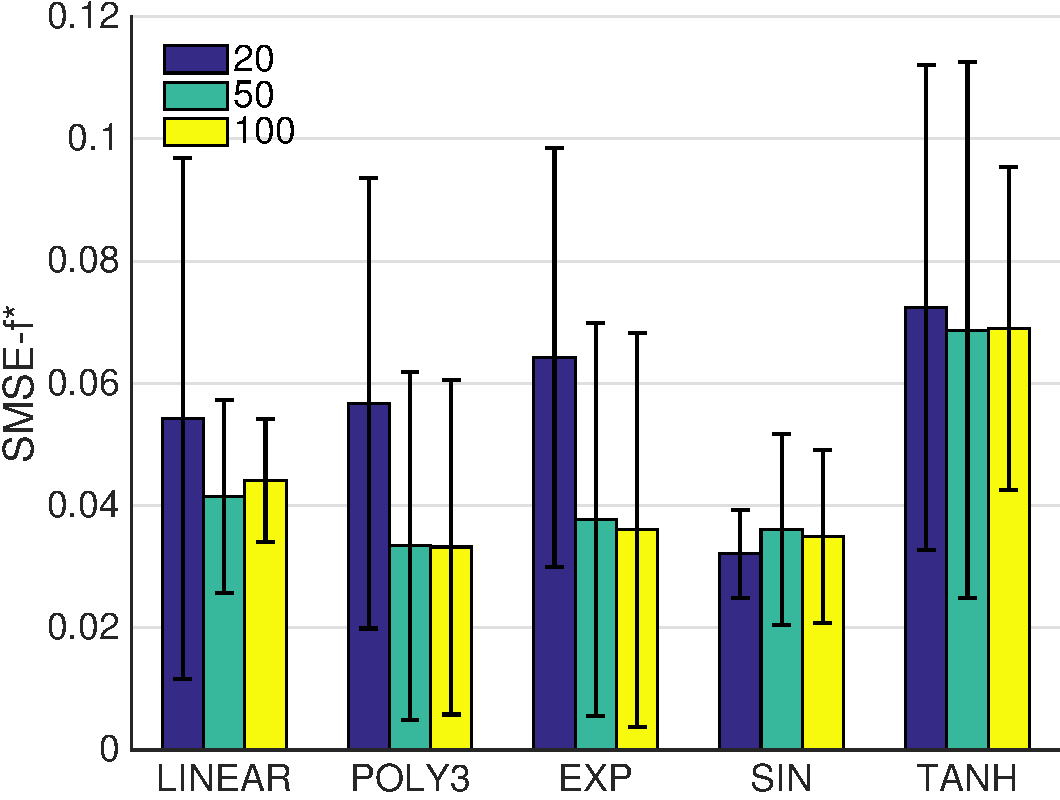
\includegraphics[width=0.31\linewidth]{toyData-EKS-SMSE-fstar} &
\includegraphics[width=0.31\linewidth]{toyData-EKS-NLPD-fstar} &
\includegraphics[width=0.31\linewidth]{toyData-EKS-SMSE-gstar} \\
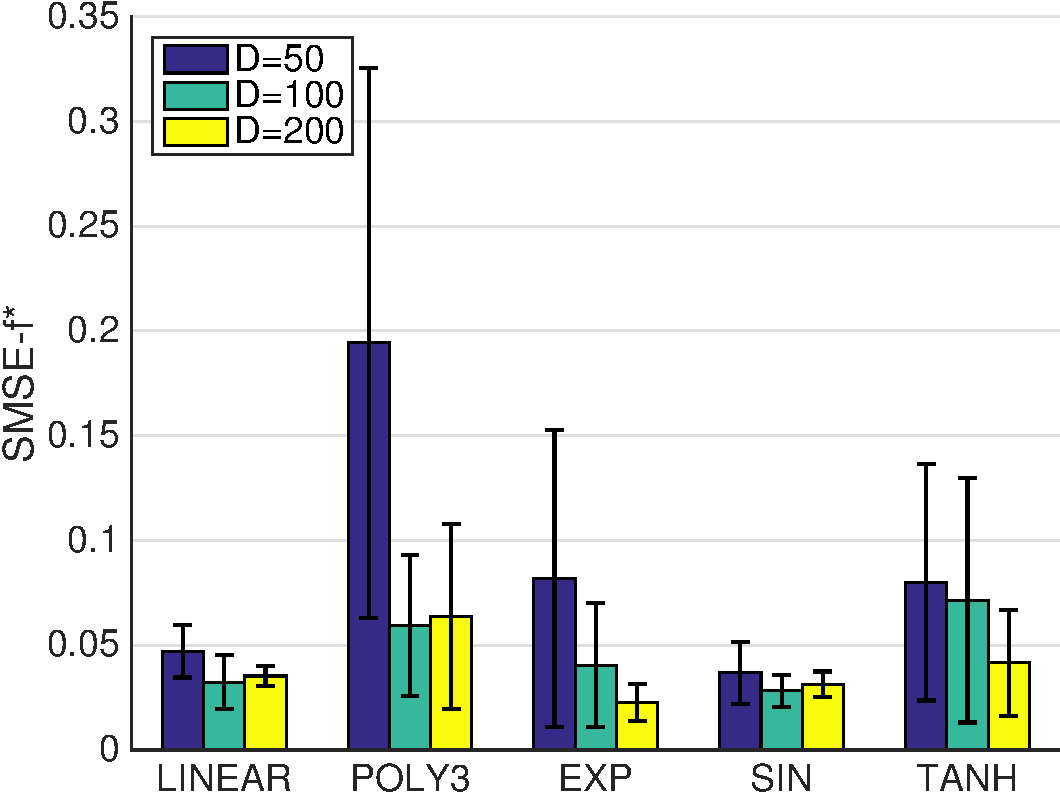
\includegraphics[width=0.31\linewidth]{toyData-UKS-SMSE-fstar} &
\includegraphics[width=0.31\linewidth]{toyData-UKS-NLPD-fstar} &
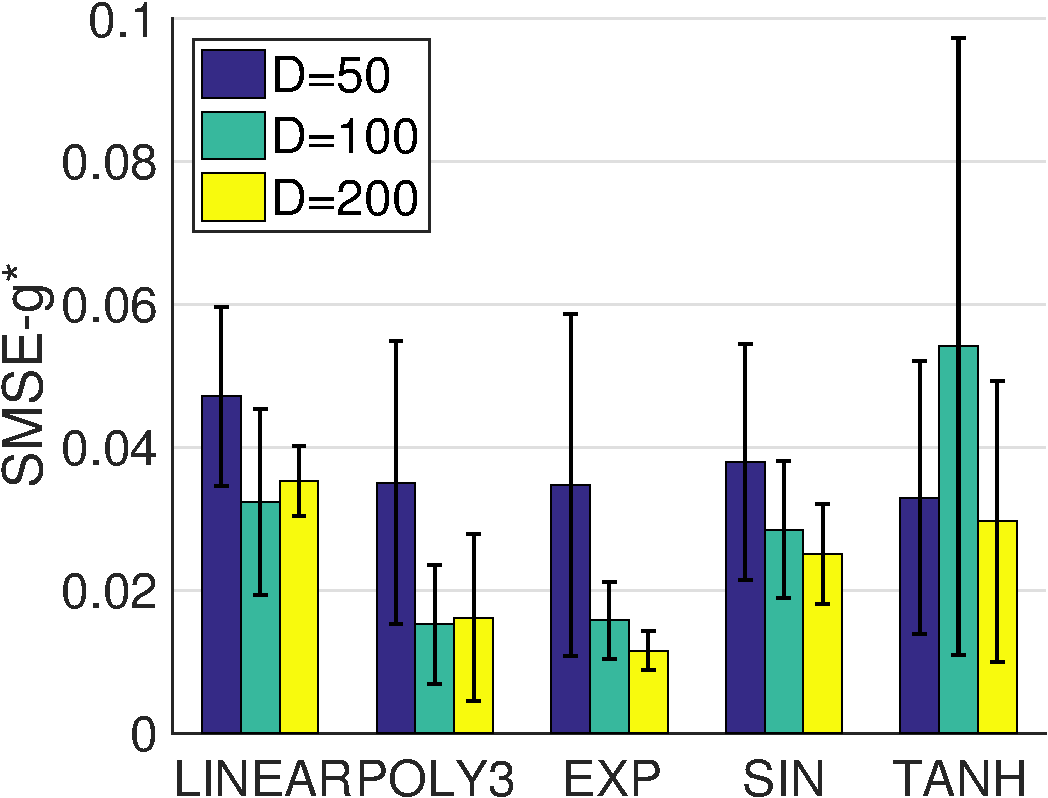
\includegraphics[width=0.31\linewidth]{toyData-UKS-SMSE-gstar} \\
\end{tabular}
\caption{The performance of the \eks (top) and \uks (bottom)
on the synthetic inversion problems as a function of the number of features used. 
\label{fig:toyinversions}
}
\end{figure*}
%
%%%%%%%
\subsection{Binary Handwritten Digit Classification}
In this experiment we re-create the second experiment from
\citet{steinberg-bonilla-nips-2014}, which is a binary classification task to
classify between images of the handwritten digits `3' and `5' in the USPS
digits datasets \cite{rasmussen-williams-book}. There are 767 images in the
training set, and 773 images in the test set. We use a logistic sigmoid as a
forward model in this task and the same settings as in the original
    experiments for covariance functions and observation variance. The main
aim of this experiment, again, is to benchmark the performance of the \eks and
\uks against the \egp and \ugp for varying numbers of basis functions, as shown
in Figure \ref{fig:usps}. 

We observe that there is a detriment in performance with a small 
number of features ($D=200$),  which is to be expected since the input image 
features have a dimension of $d = 256$, and so
the exact covariance would be harder to represent with a low number of random
basis functions. 
However, the performance of the
\eks and \uks approaches that of the \ugp and \egp with 400 basis functions,
which indicates that our random-feature approaches are reasonable approximations to
the original \gp model. More importantly, for problems with a large number of training 
points, the \egp and the \ugp are simply unfeasible, and this is the subject of discussion 
in the next section.
\begin{figure}[t]
\centering
\begin{tabular}{c c}
\includegraphics[width=0.8\linewidth]{uspsData-NLP}  \\
\includegraphics[width=0.8\linewidth]{uspsData-ERROR-RATE}  
\end{tabular}
\caption{The performance of the \eks and \uks (bottom) on the binary classification problem for the \usps dataset as a function of 
the number of  basis used. \egp and \ugp are the original (full) \gp models.
\label{fig:usps}
}
\end{figure}
%
 
%%%%%%%%%
\subsection{Large Scale Classification} 
Here we present the results of our inference algorithms on a larger application on the 
\mnist dataset, which contains examples of handwritten digits, 50,000 for training, 10,000 
for validation and 10,000 for testing. In our experiments below, we always train on 60,000 
examples that include the training and the validation set and tune the parameters of our 
models via optimization of the variational bound. This is probably a disadvantage when compare
to other approaches that use cross-validation but our goal is only to show that our models can 
achieve competitive performance at this scale. 

\textbf{Odd digits vs even digits.} We first consider the binary classification problem 
of distinguishing the odd digits vs the 
even digits, a task that has also been investigated by \cite{hensman-et-al-aistats-2015}.
The results are shown in Table \ref{tab:mnistBinary}, for our methods (\eks and \uks) and 
the methods by  \citep[][\hmg]{hensman-et-al-aistats-2015} and \citep[][\dnb]{dezfouli-bonilla-nips-2015}.
As before, we report the mean negative log probability and the error rate on the test 
set for different number of feature basis. We see that our methods achieve similar performance 
to \hmg and \dnb when using 2000 feature basis, while \dnb is an inducing-point approach that 
uses 2000 inducing points fixed via clustering, and  \hmg uses 200 inducing points with the 
extra overhead of learning their locations. 
%
\begin{table}[h]
\caption{The performance of the models on the \mnist dataset for the 
task of classifying the even digits vs the odd digits.
\label{tab:mnistBinary}
}
\begin{tabular}{c c c c c}
\toprule
& \multicolumn{2}{c}{NLP} & \multicolumn{2}{c}{Error Rate} \\
& D = 1000 & D = 2000 & D = 1000 & D = 2000 \\
\midrule
\eks &  0.129 & 0.088 & 0.043 & 0.026 \\
\uks &  0.129 & 0.088 & 0.043 & 0.026 \\
\hmg &      \multicolumn{2}{c}{0.069}    &            \multicolumn{2}{c}{0.022}   \\
\dnb   &      \multicolumn{2}{c}{0.068}    &            \multicolumn{2}{c}{0.022}\\
\bottomrule
\end{tabular}
\end{table}

\textbf{Multi-class classification:} One of the contributions of our approach with respect 
to the original \egp and \ugp models is its scalability to a large number of observations 
when having multiple outputs. In this experiment we applied our algorithm to the task
of classifying all digits on and the \eks and \uks achieved similar performance. For 
example, the \eks achieved and error rate of $ 04.75\%$ and 
a NLP of $-0.1887$, when using $D=1000$ features. When we increased the number 
of features to 	$D=2000$, it attained an error rate of 3.81\% and an NLP of $-0.1304$.
The error rates  lower than those reported by  \citet{gal-et-al-nips-2014}  and, with less 
computations, while  \citet{dezfouli-bonilla-nips-2015} reported an error 
rate of $2.51\%$. As a reference, linear classifiers achive around $12\%$ error rate on this 
task while the state of the art is less than $1\%$. 












\subsection{Seismic Inversion}

Seismic data from the Otway basin (Pretty Hill formation) is used in this
experiment. We wish to infer the geometry and layer velocity based on seismic
reflection data, and a prior on the \emph{mean depth} of the layers (constant
mean function in a GP). There are four layers in this dataset, which means $P =
4$ (travel times) and $Q = 8$ (depth of layer boundaries, layer velocities).
Will we also need a (non-zero) prior on velocities since we have more latent
tasks than output tasks??

This can be the experimental setup;
\begin{itemize}
    \item We can validate our algorithm on 1D slices of this data (about
        100--300 interpolated seismic travel times).
    \item We will use a 1D MCMC result as `ground truth' for this problem.
    \item We need to validate on 1D because MCMC cannot optimise too many knot
        points for the splines it uses to model the geometry (dimensionality is
        too high).
    \item We can also potentially compare to the simple optimisation method
        (non-probabilistic), especially if we also need to get the gradient of
        the forward model.
    \item We can then demonstrate the \eks and \uks on the whole 2D problem,
        which is inferring a $500\times300$ grid (O(100,000) points) \emph{per
            task}. We will need an SGD/SVI implementation for this.
\end{itemize}



 
